
	\section{Smoothers}
		\subsubsection{Jacobi's method}
		The implementation of the Jacobian algorithm, which was described in \cref{sec:GSRB}, is straightforward, but it has the downside of slow convergence and
		bad smoothing properties, in addition to the need of additional grid values. When \(\phi^{n+1}_{i}\) is computed
		we need access to the previous value \(\phi^n_{i-1}\), so either the previous values
		need to stored seperately, or \(\phi^{n+1}_{i}\) can be computed on a new grid and then copied over after completing the cycle.
		In this implementation we computed the solution on a temporary grid and then copied over, since it was mostly for debugging purposes in the early development, and
		efficiency was not a concern.

		The computation is done by starting at index \(g=0\), computing the surrounding grid indexes, \(gj, gjj,...\), where \(gj\)
		is the next grid point along the x-axis, and \(gjj\) is the previous value. Then the entire grid is looped trough over, incrementing
		both \(g\) and the surrounding grid indexes \(gj, gjj,...\). The computation on the ghost layers will be incorrect but those will be overwritten
		when swapping halos. As mentioned Jacobi's method was used for development and testing, but in the final version we use the Gauss-Seidel Red and Black ordering.


		\subsubsection{Gauss-Seidel Red and Black}
		In the implementation of Gauss-Seidel algorithm we use a clever ordering of the computations,
		called Red and Black ordering, both to increase the smoothing properties of the algorithm as well as avoiding
 		creating a temporary grid to store \(\phi^{n+1}\) in. Every grid point where the indexes sum up to an even number
		is labeled a red point and the odd index groupings are labeled black points, see \cref{fig:RB_ordering}. Then
		each red point is directly surrounded by only black points and vica versa.

		A cycle is then divided into 2 halfcycles, where each halfcycle computes \(\phi^{n+1}\) for the red and black points respectively.


		\begin{enumerate}
			\item for(int c = 0; c \(<\) nCycles; c++)
				\begin{itemize}
					\item Cycle through red points and compute \(\phi^{n+1}\)
					\item Swap Halo
					\item Cycle through black points and compute \(\phi^{n+1}\)
					\item Swap Halo
				\end{itemize}
		\end{enumerate}

		For the 2 dimensional case the iteration is done first for the odd rows and even rows seperately, due
		to the similarity between all the red points in the odd rows, and between the red points in the even rows.
		Then the cycling could be generalized into a static inline function used for all the cycling.

		%Figure
		\tikzstyle{red}=[circle,fill=red!70,minimum size=10pt,inner sep=0pt]
		\tikzstyle{black}=[circle,fill=black!40,minimum size=10pt,inner sep=0pt]
		\tikzstyle{ghost}=[circle,fill=blue!20,minimum size=10pt,inner sep=0pt]

		\begin{figure}
			\centering
			\begin{subfigure}[b]{0.45\textwidth}
			\centering
			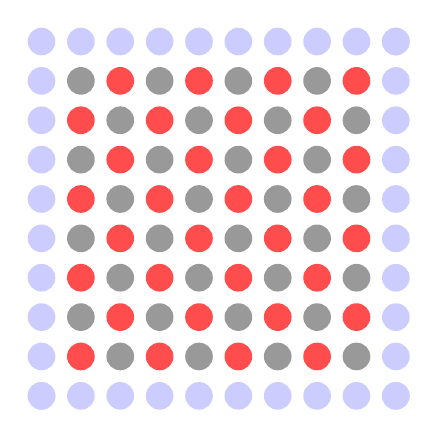
\begin{tikzpicture}[scale=0.50, auto,swap]
				%Adding the ghost nodes along the edges
				\foreach \pos/\name in 	{{(0,0)/},	{(1,0)/}, 	{(2,0)/},	{(3,0)/},
										 {(4,0)/},	{(5,0)/}, 	{(6,0)/},	{(7,0)/},
										 {(8,0)/},	{(9,0)/}}
				\node[ghost] (\name) at \pos {$\name$};
				\foreach \pos/\name in 	{			{(0,1)/}, 	{(0,2)/},		{(0,3)/},
										{(0,4)/},	{(0,5)/}, 	{(0,6)/},		{(0,7)/},
										{(0,8)/}, 	{(0,9)/}}
				\node[ghost] (\name) at \pos {$\name$};
				\foreach \pos/\name in 	{{(0,0)/},	{(1,9)/}, 	{(2,9)/},		{(3,9)/},
										 {(4,9)/},	{(5,9)/}, 	{(6,9)/},		{(7,9)/},
										 {(8,9)/}, 	{(9,9)/}}
				\node[ghost] (\name) at \pos {$\name$};
				\foreach \pos/\name in 	{{(9,0)/},	{(9,1)/}, {(9,2)/},		{(9,3)/},
										 {(9,4)/},	{(9,5)/}, {(9,6)/},		{(9,7)/},
										 {(9,8)/},	{(9,9)/}}
				\node[ghost] (\name) at \pos {$\name$};
				%The red nodes
				\foreach \pos/\name in {{(1,1)/}, 	{(2,2)/},		{(3,3)/},		{(4,4)/},
										{(5,5)/}, 	{(6,6)/},		{(7,7)/},		{(8,8)/}}
				%Above Diagonal
				\node[red] (\name) at \pos {$\name$};
				\foreach \pos/\name in {{(1,3)/}, {(2,4)/},	{(3,5)/}, {(4,6)/}, {(5,7)/}, {(6,8)/}}
				\node[red] (\name) at \pos {$\name$};
				\foreach \pos/\name in {{(1,5)/}, {(2,6)/},	{(3,7)/}, {(4,8)/}}
				\node[red] (\name) at \pos {$\name$};
				\foreach \pos/\name in {{(1,7)/}, {(2,8)/}}
				\node[red] (\name) at \pos {$\name$};
				%Below Diagonal
				\foreach \pos/\name in {{(3,1)/}, {(4,2)/},	{(5,3)/}, {(6,4)/}, {(7,5)/}, {(8,6)/}}
				\node[red] (\name) at \pos {$\name$};
				\foreach \pos/\name in {{(5,1)/}, {(6,2)/},	{(7,3)/}, {(8,4)/}}
				\node[red] (\name) at \pos {$\name$};
				\foreach \pos/\name in {{(7,1)/}, {(8,2)/}}
				\node[red] (\name) at \pos {$\name$};
				%Black nodes
				%Above diagonal
				\foreach \pos/\name in {{(1,2)/}, 	{(2,3)/},		{(3,4)/},		{(4,5)/},
										{(5,6)/}, 	{(6,7)/},		{(7,8)/}}
				\node[black] (\name) at \pos {$\name$};
				\foreach \pos/\name in {{(1,4)/}, 	{(2,5)/},		{(3,6)/},		{(4,7)/},
										{(5,8)/}}
				\node[black] (\name) at \pos {$\name$};
				\foreach \pos/\name in {{(1,6)/}, 	{(2,7)/},		{(3,8)/}}
				\node[black] (\name) at \pos {$\name$};
				\foreach \pos/\name in {{(1,8)/}}
				\node[black] (\name) at \pos {$\name$};
				%Below diagonal
				\foreach \pos/\name in {{(2,1)/},	{(3,2)/},	{(4,3)/},	{(5,4)/},
 										{(6,5)/},	{(7,6)/}, 	{(8,7)/}}
				\node[black] (\name) at \pos {$\name$};
				\foreach \pos/\name in {{(4,1)/},	{(5,2)/},	{(6,3)/},	{(7,4)/},	{(8,5)/}}
				\node[black] (\name) at \pos {$\name$};
				\foreach \pos/\name in {{(6,1)/},	{(7,2)/},	{(8,3)/}}
				\node[black] (\name) at \pos {$\name$};
				\foreach \pos/\name in {{(8,1)/}}
				\node[black] (\name) at \pos {$\name$};
			\end{tikzpicture}
			\caption{This figure shows the Red and Black ordering, utlized by the GS-RB algorithm. Each color is done seperately.}
			\label{fig:RB_ordering}
			\end{subfigure}
	\end{figure}

	For the 3 dimensional case there are two different approaches to the problem, one where the iteration through the grid is streamlined, but needs
	several loops through the grid to take care of a subset of the grid points each loop. The other algorithm uses one loop through the grid,
	with different conditions on the edges to make it go through the correct grid points in each line.

	When the loops are streamlined the edges the loop go through the entire grid, but when it reaches and edge in it either needs to add or subtract \(1\) to
	the iterator index. In \label{eq:RB_loop} we want to do a red pass, computing all the red values, the grid is cycled through increasing by 2 each time.
	Then it will access up the indexes, \(36, 38, 40,42, \cdots\). In the second row we want it to use the index \(43\), instead of \(42\), so we need to
	increase it by \(1\) when it reaches the edge. When it reaches the end of the second line, we want it to increase from \(47\) to \(48\),
	so then we need to subtract \(1\). In the next layer we need to shift the behaviour on the edges to the opposite.

	\[
	\begin{matrix}
	.	&	.	&	. &	.	& .	& .
	\\
	\textcolor{red}{48} &49 &\textcolor{red}{49} &50 & \textcolor{red}{51} &52
	\\
	42	& \textcolor{red}{43} &44 &\textcolor{red}{45} &46 &\textcolor{red}{47}
	\\
	\textcolor{red}{36} & 37 &\textcolor{red}{38}  &39 & \textcolor{red}{40} & 41
	\end{matrix}
	\label{eq:RB-loop}
	\]

	In the other implementation I tried something similar to the 2D implementation, where it does several
	loops through the grid, computing an easier subgroup of the red nodes each time, so the iteratior index
	can increase by just to each time. So for the red points it computes the odd and even layers and rows seperately.

	\begin{itemize}
		\item Compute Odd layers, odd rows
		\item Compute Odd layers, even rows
		\item Compute Even Layers, odd rows
		\item Compute Even layers, even rows
	\end{itemize}


	% \newpage
	% \subsection{Jacobian code}
	% \label{sec:jacobian}
	%
	% \begin{lstlisting}[language=c, caption = Code snippet 2D jacobian]
	% 	for(int c = 0; c < nCycles; c++){
	% 		// Index of neighboring nodes
	% 		int gj = sizeProd[1];
	% 		int gjj= -sizeProd[1];
	% 		int gk = sizeProd[2];
	% 		int gkk= -sizeProd[2];
	%
	% 		for(long int g = 0; g < sizeProd[rank]; g++){
	% 			tempVal[g] = 0.25*(	phiVal[gj] + phiVal[gjj] +
	% 								phiVal[gk] + phiVal[gkk] + rhoVal[g]);
	%
	% 			gj++;
	% 			gjj++;
	% 			gk++;
	% 			gkk++;
	% 		}
	%
	% 		for(int q = 0; q < sizeProd[rank]; q++) phiVal[q] = tempVal[q];
	% 		for(int d = 1; d < rank; d++) gSwapHalo(phi, mpiInfo, d);
	% 	}
	% \end{lstlisting}

	% \newpage
	% \subsection{GS-RB 2D}
	% \label{sec:GS_RB_2D}
	% \begin{lstlisting}[language=c, caption = Main loop]
	% 		for(int c = 0; c < nCycles;c++){
	%
	% 			//Increments
	% 			int kEdgeInc = nGhostLayers[2] + nGhostLayers[rank + 2] + sizeProd[2];
	%
	% 			/**************************
	% 			 *	Red Pass
	% 			 *************************/
	% 			//Odd numbered rows
	% 			g = nGhostLayers[1] + sizeProd[2];
	% 			loopRedBlack2D(rhoVal, phiVal, sizeProd, trueSize, kEdgeInc, g, gj, gjj, gk, gkk);
	%
	% 			//Even numbered columns
	% 			g = nGhostLayers[1] + 1 + 2*sizeProd[2];
	% 			loopRedBlack2D(rhoVal, phiVal, sizeProd, trueSize, kEdgeInc, g, gj, gjj, gk, gkk);
	%
	% 			for(int d = 1; d < rank; d++) gSwapHalo(phi, mpiInfo, d);
	%
	% 			/***********************************
	% 			 *	Black pass
	% 			 **********************************/
	% 			//Odd numbered rows
	% 			g = nGhostLayers[1] + 1 + sizeProd[2];
	% 			loopRedBlack2D(rhoVal, phiVal, sizeProd, trueSize, kEdgeInc, g, gj, gjj, gk, gkk);
	%
	% 			//Even numbered columns
	% 			g = nGhostLayers[1] + 2*sizeProd[2];
	% 			loopRedBlack2D(rhoVal, phiVal, sizeProd, trueSize, kEdgeInc, g, gj, gjj, gk, gkk);
	%
	%
	% 			for(int d = 1; d < rank; d++) gSwapHalo(phi, mpiInfo, d);
	% 		}
	%
	% 		return;
	% 	}
	% \end{lstlisting}

	% \begin{lstlisting}[language=c, caption = Loop through grid]
	% 	gj = g + sizeProd[1];
	% 	gjj= g - sizeProd[1];
	% 	gk = g + sizeProd[2];
	% 	gkk= g - sizeProd[2];
	%
	% 	for(int k = 1; k < trueSize[2]; k +=2){
	% 		for(int j = 1; j < trueSize[1]; j += 2){
	% 			phiVal[g] = 0.25*(	phiVal[gj] + phiVal[gjj] +
	% 								phiVal[gk] + phiVal[gkk] + rhoVal[g]);
	% 			g	+=2;
	% 			gj	+=2;
	% 			gjj	+=2;
	% 			gk	+=2;
	% 			gkk	+=2;
	% 		}
	% 		g	+=kEdgeInc;
	% 		gj	+=kEdgeInc;
	% 		gjj	+=kEdgeInc;
	% 		gk	+=kEdgeInc;
	% 		gkk	+=kEdgeInc;
	% 	}
	% \end{lstlisting}

	% \newpage
	% \section{GS-RB 3D if tests}
	% \label{sec:GS-RB_if}
	% \begin{lstlisting}[language=c, caption = GS-RB with if-tests]
	%
	% 	/*********************
	% 	 *	Red Pass
	% 	 ********************/
	% 	g = sizeProd[3]*nGhostLayers[3];
	% 	for(int l = 0; l < trueSize[3];l++){
	% 		for(int k = 0; k < size[2]; k++){
	% 			for(int j = 0; j < size[1]; j+=2){
	% 				phiVal[g] = 0.125*(	phiVal[g+gj] + phiVal[g-gj] +
	% 									phiVal[g+gk] + phiVal[g-gk] +
	% 									phiVal[g+gl] + phiVal[g-gl] + rhoVal[g]);
	% 				g	+=2;
	% 			}
	% 			if(l%2){
	% 				if(k%2)	g+=1; else g-=1;
	% 			} else {
	% 				if(k%2) g-=1; else g+=1;
	% 			}
	%
	% 		}
	% 		if(l%2) g-=1; else g+=1;
	% 	}
	%
	% 	for(int d = 1; d < rank; d++) gSwapHalo(phi, mpiInfo, d);
	% \end{lstlisting}

	% \newpage
	% \section{GS-RB 3D without if tests}
	% \begin{lstlisting}[language=c, caption = main routine]
	% /**************************
	%  *	Red Pass
	%  *************************/
	% //Odd layers - Odd Rows
	% g = nGhostLayers[1]*sizeProd[1] + nGhostLayers[2]*sizeProd[2] + nGhostLayers[3]*sizeProd[3];
	% loopRedBlack3D(rhoVal, phiVal, sizeProd, trueSize, kEdgeInc, lEdgeInc,
	% 				g, gj, gjj, gk, gkk, gl, gll);
	%
	% //Odd layers - Even Rows
	% g = (nGhostLayers[1]+1)*sizeProd[1] + (nGhostLayers[2]+1)*sizeProd[2] + nGhostLayers[3]*sizeProd[3];
	% loopRedBlack3D(rhoVal, phiVal, sizeProd, trueSize, kEdgeInc, lEdgeInc,
	% 				g, gj, gjj, gk, gkk, gl, gll);
	%
	% //Even layers - Odd Rows
	% g = (nGhostLayers[1])*sizeProd[1] + (nGhostLayers[2])*sizeProd[2] + (nGhostLayers[3]+1)*sizeProd[3];
	% loopRedBlack3D(rhoVal, phiVal, sizeProd, trueSize, kEdgeInc, lEdgeInc,
	% 				g, gj, gjj, gk, gkk, gl, gll);
	%
	% //Even layers - Even Rows
	% g = (nGhostLayers[1] + 1)*sizeProd[1] + (nGhostLayers[2]+1)*sizeProd[2] + (nGhostLayers[3]+1)*sizeProd[3];
	% loopRedBlack3D(rhoVal, phiVal, sizeProd, trueSize, kEdgeInc, lEdgeInc,
	% 				g, gj, gjj, gk, gkk, gl, gll);
	%
	% for(int d = 1; d < rank; d++) gSwapHalo(phi, mpiInfo, d);
	% \end{lstlisting}
	%
	% \begin{lstlisting}[language=c, caption = loop routine]
	% 	inline static void loopRedBlack3D(double *rhoVal,double *phiVal,long int *sizeProd, int *trueSize, int kEdgeInc, int lEdgeInc,
	% 				long int g, long int gj, long int gjj, long int gk, long int gkk, long int gl, long int gll){
	%
	% 	gj = g + sizeProd[1];
	% 	gjj= g - sizeProd[1];
	% 	gk = g + sizeProd[2];
	% 	gkk= g - sizeProd[2];
	% 	gl = g + sizeProd[3];
	% 	gll= g - sizeProd[3];
	%
	% 	for(int l = 0; l<trueSize[3]; l+=2){
	% 		for(int k = 0; k < trueSize[2]; k+=2){
	% 			for(int j = 0; j < trueSize[1]; j+=2){
	% 				// msg(STATUS, "g=%d", g);
	% 				phiVal[g] = 0.125*(phiVal[gj] + phiVal[gjj] +
	% 								phiVal[gk] + phiVal[gkk] +
	% 								phiVal[gl] + phiVal[gll] + rhoVal[g]);
	% 				g	+=2;
	% 				gj	+=2;
	% 				gjj	+=2;
	% 				gk	+=2;
	% 				gkk	+=2;
	% 				gl	+=2;
	% 				gll	+=2;{subfigure}
	% 			}
	% 		g	+=kEdgeInc;
	% 		gj	+=kEdgeInc;
	% 		gjj	+=kEdgeInc;
	% 		gk	+=kEdgeInc;
	% 		gkk	+=kEdgeInc;
	% 		gl	+=kEdgeInc;
	% 		gll	+=kEdgeInc;
	% 		}
	% 	g	+=lEdgeInc;
	% 	gj	+=lEdgeInc;
	% 	gjj	+=lEdgeInc;
	% 	gk	+=lEdgeInc;
	% 	gkk	+=lEdgeInc;
	% 	gl	+=lEdgeInc;
	% 	gll	+=lEdgeInc;
	% 	}
	%
	% 	return;
	% }
	%
	% \end{lstlisting}
